% Options for packages loaded elsewhere
\PassOptionsToPackage{unicode}{hyperref}
\PassOptionsToPackage{hyphens}{url}
\PassOptionsToPackage{dvipsnames,svgnames,x11names}{xcolor}
%
\documentclass[
  letterpaper,
  DIV=11,
  numbers=noendperiod]{scrartcl}

\usepackage{amsmath,amssymb}
\usepackage{iftex}
\ifPDFTeX
  \usepackage[T1]{fontenc}
  \usepackage[utf8]{inputenc}
  \usepackage{textcomp} % provide euro and other symbols
\else % if luatex or xetex
  \usepackage{unicode-math}
  \defaultfontfeatures{Scale=MatchLowercase}
  \defaultfontfeatures[\rmfamily]{Ligatures=TeX,Scale=1}
\fi
\usepackage{lmodern}
\ifPDFTeX\else  
    % xetex/luatex font selection
\fi
% Use upquote if available, for straight quotes in verbatim environments
\IfFileExists{upquote.sty}{\usepackage{upquote}}{}
\IfFileExists{microtype.sty}{% use microtype if available
  \usepackage[]{microtype}
  \UseMicrotypeSet[protrusion]{basicmath} % disable protrusion for tt fonts
}{}
\makeatletter
\@ifundefined{KOMAClassName}{% if non-KOMA class
  \IfFileExists{parskip.sty}{%
    \usepackage{parskip}
  }{% else
    \setlength{\parindent}{0pt}
    \setlength{\parskip}{6pt plus 2pt minus 1pt}}
}{% if KOMA class
  \KOMAoptions{parskip=half}}
\makeatother
\usepackage{xcolor}
\setlength{\emergencystretch}{3em} % prevent overfull lines
\setcounter{secnumdepth}{-\maxdimen} % remove section numbering
% Make \paragraph and \subparagraph free-standing
\makeatletter
\ifx\paragraph\undefined\else
  \let\oldparagraph\paragraph
  \renewcommand{\paragraph}{
    \@ifstar
      \xxxParagraphStar
      \xxxParagraphNoStar
  }
  \newcommand{\xxxParagraphStar}[1]{\oldparagraph*{#1}\mbox{}}
  \newcommand{\xxxParagraphNoStar}[1]{\oldparagraph{#1}\mbox{}}
\fi
\ifx\subparagraph\undefined\else
  \let\oldsubparagraph\subparagraph
  \renewcommand{\subparagraph}{
    \@ifstar
      \xxxSubParagraphStar
      \xxxSubParagraphNoStar
  }
  \newcommand{\xxxSubParagraphStar}[1]{\oldsubparagraph*{#1}\mbox{}}
  \newcommand{\xxxSubParagraphNoStar}[1]{\oldsubparagraph{#1}\mbox{}}
\fi
\makeatother

\usepackage{color}
\usepackage{fancyvrb}
\newcommand{\VerbBar}{|}
\newcommand{\VERB}{\Verb[commandchars=\\\{\}]}
\DefineVerbatimEnvironment{Highlighting}{Verbatim}{commandchars=\\\{\}}
% Add ',fontsize=\small' for more characters per line
\usepackage{framed}
\definecolor{shadecolor}{RGB}{241,243,245}
\newenvironment{Shaded}{\begin{snugshade}}{\end{snugshade}}
\newcommand{\AlertTok}[1]{\textcolor[rgb]{0.68,0.00,0.00}{#1}}
\newcommand{\AnnotationTok}[1]{\textcolor[rgb]{0.37,0.37,0.37}{#1}}
\newcommand{\AttributeTok}[1]{\textcolor[rgb]{0.40,0.45,0.13}{#1}}
\newcommand{\BaseNTok}[1]{\textcolor[rgb]{0.68,0.00,0.00}{#1}}
\newcommand{\BuiltInTok}[1]{\textcolor[rgb]{0.00,0.23,0.31}{#1}}
\newcommand{\CharTok}[1]{\textcolor[rgb]{0.13,0.47,0.30}{#1}}
\newcommand{\CommentTok}[1]{\textcolor[rgb]{0.37,0.37,0.37}{#1}}
\newcommand{\CommentVarTok}[1]{\textcolor[rgb]{0.37,0.37,0.37}{\textit{#1}}}
\newcommand{\ConstantTok}[1]{\textcolor[rgb]{0.56,0.35,0.01}{#1}}
\newcommand{\ControlFlowTok}[1]{\textcolor[rgb]{0.00,0.23,0.31}{\textbf{#1}}}
\newcommand{\DataTypeTok}[1]{\textcolor[rgb]{0.68,0.00,0.00}{#1}}
\newcommand{\DecValTok}[1]{\textcolor[rgb]{0.68,0.00,0.00}{#1}}
\newcommand{\DocumentationTok}[1]{\textcolor[rgb]{0.37,0.37,0.37}{\textit{#1}}}
\newcommand{\ErrorTok}[1]{\textcolor[rgb]{0.68,0.00,0.00}{#1}}
\newcommand{\ExtensionTok}[1]{\textcolor[rgb]{0.00,0.23,0.31}{#1}}
\newcommand{\FloatTok}[1]{\textcolor[rgb]{0.68,0.00,0.00}{#1}}
\newcommand{\FunctionTok}[1]{\textcolor[rgb]{0.28,0.35,0.67}{#1}}
\newcommand{\ImportTok}[1]{\textcolor[rgb]{0.00,0.46,0.62}{#1}}
\newcommand{\InformationTok}[1]{\textcolor[rgb]{0.37,0.37,0.37}{#1}}
\newcommand{\KeywordTok}[1]{\textcolor[rgb]{0.00,0.23,0.31}{\textbf{#1}}}
\newcommand{\NormalTok}[1]{\textcolor[rgb]{0.00,0.23,0.31}{#1}}
\newcommand{\OperatorTok}[1]{\textcolor[rgb]{0.37,0.37,0.37}{#1}}
\newcommand{\OtherTok}[1]{\textcolor[rgb]{0.00,0.23,0.31}{#1}}
\newcommand{\PreprocessorTok}[1]{\textcolor[rgb]{0.68,0.00,0.00}{#1}}
\newcommand{\RegionMarkerTok}[1]{\textcolor[rgb]{0.00,0.23,0.31}{#1}}
\newcommand{\SpecialCharTok}[1]{\textcolor[rgb]{0.37,0.37,0.37}{#1}}
\newcommand{\SpecialStringTok}[1]{\textcolor[rgb]{0.13,0.47,0.30}{#1}}
\newcommand{\StringTok}[1]{\textcolor[rgb]{0.13,0.47,0.30}{#1}}
\newcommand{\VariableTok}[1]{\textcolor[rgb]{0.07,0.07,0.07}{#1}}
\newcommand{\VerbatimStringTok}[1]{\textcolor[rgb]{0.13,0.47,0.30}{#1}}
\newcommand{\WarningTok}[1]{\textcolor[rgb]{0.37,0.37,0.37}{\textit{#1}}}

\providecommand{\tightlist}{%
  \setlength{\itemsep}{0pt}\setlength{\parskip}{0pt}}\usepackage{longtable,booktabs,array}
\usepackage{calc} % for calculating minipage widths
% Correct order of tables after \paragraph or \subparagraph
\usepackage{etoolbox}
\makeatletter
\patchcmd\longtable{\par}{\if@noskipsec\mbox{}\fi\par}{}{}
\makeatother
% Allow footnotes in longtable head/foot
\IfFileExists{footnotehyper.sty}{\usepackage{footnotehyper}}{\usepackage{footnote}}
\makesavenoteenv{longtable}
\usepackage{graphicx}
\makeatletter
\newsavebox\pandoc@box
\newcommand*\pandocbounded[1]{% scales image to fit in text height/width
  \sbox\pandoc@box{#1}%
  \Gscale@div\@tempa{\textheight}{\dimexpr\ht\pandoc@box+\dp\pandoc@box\relax}%
  \Gscale@div\@tempb{\linewidth}{\wd\pandoc@box}%
  \ifdim\@tempb\p@<\@tempa\p@\let\@tempa\@tempb\fi% select the smaller of both
  \ifdim\@tempa\p@<\p@\scalebox{\@tempa}{\usebox\pandoc@box}%
  \else\usebox{\pandoc@box}%
  \fi%
}
% Set default figure placement to htbp
\def\fps@figure{htbp}
\makeatother

\KOMAoption{captions}{tableheading}
\makeatletter
\@ifpackageloaded{caption}{}{\usepackage{caption}}
\AtBeginDocument{%
\ifdefined\contentsname
  \renewcommand*\contentsname{Table of contents}
\else
  \newcommand\contentsname{Table of contents}
\fi
\ifdefined\listfigurename
  \renewcommand*\listfigurename{List of Figures}
\else
  \newcommand\listfigurename{List of Figures}
\fi
\ifdefined\listtablename
  \renewcommand*\listtablename{List of Tables}
\else
  \newcommand\listtablename{List of Tables}
\fi
\ifdefined\figurename
  \renewcommand*\figurename{Figure}
\else
  \newcommand\figurename{Figure}
\fi
\ifdefined\tablename
  \renewcommand*\tablename{Table}
\else
  \newcommand\tablename{Table}
\fi
}
\@ifpackageloaded{float}{}{\usepackage{float}}
\floatstyle{ruled}
\@ifundefined{c@chapter}{\newfloat{codelisting}{h}{lop}}{\newfloat{codelisting}{h}{lop}[chapter]}
\floatname{codelisting}{Listing}
\newcommand*\listoflistings{\listof{codelisting}{List of Listings}}
\makeatother
\makeatletter
\makeatother
\makeatletter
\@ifpackageloaded{caption}{}{\usepackage{caption}}
\@ifpackageloaded{subcaption}{}{\usepackage{subcaption}}
\makeatother

\usepackage{bookmark}

\IfFileExists{xurl.sty}{\usepackage{xurl}}{} % add URL line breaks if available
\urlstyle{same} % disable monospaced font for URLs
\hypersetup{
  pdftitle={Apuntes},
  colorlinks=true,
  linkcolor={blue},
  filecolor={Maroon},
  citecolor={Blue},
  urlcolor={Blue},
  pdfcreator={LaTeX via pandoc}}


\title{Apuntes}
\author{}
\date{}

\begin{document}
\maketitle


\section{Clase 01}\label{clase-01}

Se instala paquete kittyR.

\begin{Shaded}
\begin{Highlighting}[]
\CommentTok{\#install.packages("kittyR")}
\FunctionTok{library}\NormalTok{(kittyR)}

\CommentTok{\# Instalar paquete kittyR: https://indrajeetpatil.github.io/kittyR/, no funciona!}

\CommentTok{\#install.packages("remotes")}
\CommentTok{\#remotes::install\_github("IndrajeetPatil/kittyR")}

\FunctionTok{kittyR}\NormalTok{(}\AttributeTok{meow =} \ConstantTok{TRUE}\NormalTok{)}
\end{Highlighting}
\end{Shaded}

\pandocbounded{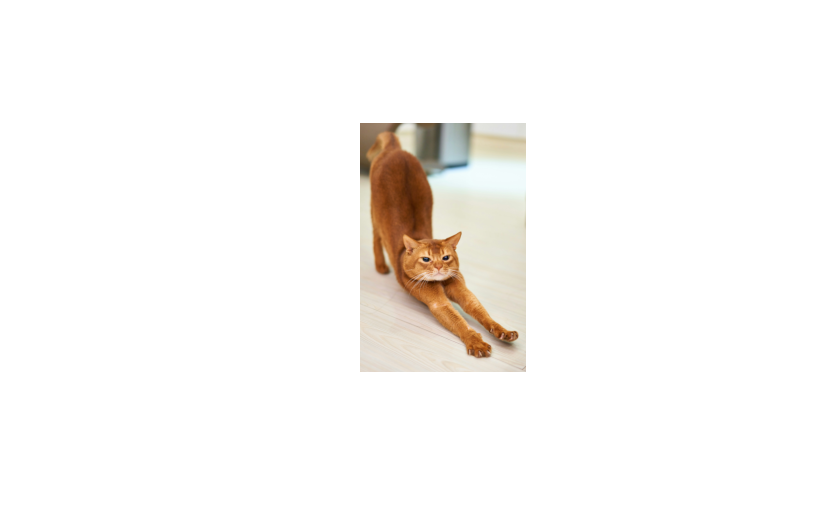
\includegraphics[keepaspectratio]{curso_programacion_r_files/figure-pdf/unnamed-chunk-1-1.pdf}}

\section{Clase 02}\label{clase-02}

\subsection{Introducción}\label{introducciuxf3n}

\begin{itemize}
\tightlist
\item
  Software libre y gratuito, su lincencia. La comunidad crea
  herramientas/paquetes colaborativas gratuitamente.
\item
  Se pueden instalar paquetes desde diferentes fuentes (CRAN, GitHub,
  BioConductor, etc).
\item
  R es sensible a mayúsculas y minúsculas! Y no lo es a los espacios
  dentro de código, pero sí dentro de bases de datos.
\item
  Valor datos faltantes: NA
\end{itemize}

\subsection{Operadores}\label{operadores}

Los más básicos

\begin{longtable}[]{@{}lll@{}}
\caption{Operadores básicos en R}\tabularnewline
\toprule\noalign{}
operador & descripcion & comentario \\
\midrule\noalign{}
\endfirsthead
\toprule\noalign{}
operador & descripcion & comentario \\
\midrule\noalign{}
\endhead
\bottomrule\noalign{}
\endlastfoot
+ & más & ojo, en ggplot es sumar capas \\
\textgreater{} & mayor & \\
\textless{} & menor & \\
\textgreater= & mayor o igual & \\
\textless= & menor o igual & \\
== & igual exacto & \\
= & igual & \\
!= & no igual & \\
! & no & \\
\textbar{} & o & \\
\& & y & \\
\%in\% & en un set & \\
\end{longtable}

\subsection{Tidyverse}\label{tidyverse}

\begin{itemize}
\tightlist
\item
  Es un gran paquete que incluye muchos paquetes, diseñados para hacer
  ciencia de datos.
\item
  Con el pipe podemos concatenar sin hacer objetos intermedios
  (\%\textgreater\%).
\item
  Buscar atajos del teclado.
\end{itemize}

\subsubsection{Importar datos}\label{importar-datos}

\begin{itemize}
\tightlist
\item
  Haven -\textgreater{} Ingresa datos de programas externos (matblab,
  stata, otros tipos de lenguajes de programación o software
  estadísticos que guarda archivos específicos).
\item
  readr -\textgreater{} Para archivos de texto (.txt)
\item
  readcl -\textgreater{} Para .xlsx
\end{itemize}

\subsubsection{Intermedio}\label{intermedio}

\begin{itemize}
\tightlist
\item
  tidyr -\textgreater{} De formato ancho a largo, etc.
\end{itemize}

\subsubsection{Transformar}\label{transformar}

\begin{itemize}
\tightlist
\item
  dplyr -\textgreater{} Transformar
\item
  purrr -\textgreater{} bucles, iteraciones, lo simplifica
\item
  broom -\textgreater{} Para hacer modelación
\item
  ggplot2 -\textgreater{} visualización datos
\end{itemize}

\subsubsection{Comunicar datos}\label{comunicar-datos}

\begin{itemize}
\tightlist
\item
  knitr
\item
  markdown -\textgreater{} reportes, presentaciones, etc.
\end{itemize}

\subsubsection{Para trabajar de
dataframes}\label{para-trabajar-de-dataframes}

\begin{itemize}
\tightlist
\item
  tibble
\item
  forcats -\textgreater{} categoricos, factores
\item
  stringr
\end{itemize}

\subsection{Terminal}\label{terminal}

Es lo que se comunica con el computador. MINGW64 escribimos como si
estuvieramos en linux, es diferente entre linux, mc y windows.

\subsection{Packages}\label{packages}

Abajo a la derecha, se ven todos los paquetes instalados. También si
está marcado es porque está cargado (library()), sino no.

\begin{Shaded}
\begin{Highlighting}[]
\FunctionTok{library}\NormalTok{(ggplot2)}
\FunctionTok{library}\NormalTok{(plotly)}

\NormalTok{p }\OtherTok{\textless{}{-}} \FunctionTok{ggplot}\NormalTok{(iris, }\FunctionTok{aes}\NormalTok{(}\AttributeTok{x =}\NormalTok{ Sepal.Length, }\AttributeTok{y =}\NormalTok{ Petal.Length, }\AttributeTok{colour =}\NormalTok{ Species)) }\SpecialCharTok{+}
  \FunctionTok{geom\_point}\NormalTok{()}

\CommentTok{\#plotly(p)}
\CommentTok{\# ojo, sale error!}
\end{Highlighting}
\end{Shaded}

\subsection{Apuntes}\label{apuntes}

\begin{itemize}
\tightlist
\item
  setwd() es para directorio de trabajo, ya no se utiliza!
\item
  Es importante que busque atajos del teclado, para hacer chuncks, hacer
  el pipe, etc.
\end{itemize}

\begin{Shaded}
\begin{Highlighting}[]
\FunctionTok{library}\NormalTok{(tidyverse)}

\CommentTok{\# Cargar con RBase:}
\NormalTok{pin1 }\OtherTok{\textless{}{-}} \FunctionTok{read.csv}\NormalTok{(}\StringTok{"datos/pinguinos.csv"}\NormalTok{)}

\CommentTok{\# Cargar con tidyverse:}
\NormalTok{pin2 }\OtherTok{\textless{}{-}} \FunctionTok{read\_csv}\NormalTok{(}\StringTok{"datos/pinguinos.csv"}\NormalTok{)}

\CommentTok{\# Cargar directamente desde github:}
\NormalTok{pin3 }\OtherTok{\textless{}{-}} \FunctionTok{read\_csv}\NormalTok{(}\StringTok{"https://raw.githubusercontent.com/rladieschile/taller{-}regex{-}2021/refs/heads/main/datos/pinguinos.csv"}\NormalTok{)}

\NormalTok{pin }\OtherTok{\textless{}{-}}\NormalTok{ pin2}
\end{Highlighting}
\end{Shaded}

\subsection{Funciones básicas}\label{funciones-buxe1sicas}

\begin{itemize}
\tightlist
\item
  select() -\textgreater{} Permite seleccionar \textbf{COLUMNAS}.
\end{itemize}

\begin{Shaded}
\begin{Highlighting}[]
\FunctionTok{select}\NormalTok{(pin, }\SpecialCharTok{{-}}\NormalTok{sexo) }\CommentTok{\#las quiero todas menos la columna sexo.}
\end{Highlighting}
\end{Shaded}

\begin{verbatim}
# A tibble: 344 x 7
   especie isla  largo_pico_mm alto_pico_mm largo_aleta_mm masa_corporal_g  anio
   <chr>   <chr>         <dbl>        <dbl>          <dbl>           <dbl> <dbl>
 1 Adelia  Torg~          39.1         18.7            181            3750  2007
 2 Adelia  Torg~          39.5         17.4            186            3800  2007
 3 Adelia  Torg~          40.3         18              195            3250  2007
 4 Adelia  Torg~          NA           NA               NA              NA  2007
 5 Adelia  Torg~          36.7         19.3            193            3450  2007
 6 Adelia  Torg~          39.3         20.6            190            3650  2007
 7 Adelia  Torg~          38.9         17.8            181            3625  2007
 8 Adelia  Torg~          39.2         19.6            195            4675  2007
 9 Adelia  Torg~          34.1         18.1            193            3475  2007
10 Adelia  Torg~          42           20.2            190            4250  2007
# i 334 more rows
\end{verbatim}

\begin{Shaded}
\begin{Highlighting}[]
\FunctionTok{select}\NormalTok{(pin, largo\_pico\_mm}\SpecialCharTok{:}\NormalTok{masa\_corporal\_g) }\CommentTok{\#selecciona columnas solo desde largo de pico hasta masa corporal}
\end{Highlighting}
\end{Shaded}

\begin{verbatim}
# A tibble: 344 x 4
   largo_pico_mm alto_pico_mm largo_aleta_mm masa_corporal_g
           <dbl>        <dbl>          <dbl>           <dbl>
 1          39.1         18.7            181            3750
 2          39.5         17.4            186            3800
 3          40.3         18              195            3250
 4          NA           NA               NA              NA
 5          36.7         19.3            193            3450
 6          39.3         20.6            190            3650
 7          38.9         17.8            181            3625
 8          39.2         19.6            195            4675
 9          34.1         18.1            193            3475
10          42           20.2            190            4250
# i 334 more rows
\end{verbatim}

\begin{Shaded}
\begin{Highlighting}[]
\FunctionTok{select}\NormalTok{(pin, sexo, isla) }\CommentTok{\#acá seleccioné solo 2 columnas, sexo e isla}
\end{Highlighting}
\end{Shaded}

\begin{verbatim}
# A tibble: 344 x 2
   sexo   isla     
   <chr>  <chr>    
 1 macho  Torgersen
 2 hembra Torgersen
 3 hembra Torgersen
 4 <NA>   Torgersen
 5 hembra Torgersen
 6 macho  Torgersen
 7 hembra Torgersen
 8 macho  Torgersen
 9 <NA>   Torgersen
10 <NA>   Torgersen
# i 334 more rows
\end{verbatim}

\begin{Shaded}
\begin{Highlighting}[]
\CommentTok{\# CON PIPE:}
\NormalTok{pin }\SpecialCharTok{\%\textgreater{}\%} \FunctionTok{select}\NormalTok{(}\SpecialCharTok{{-}}\NormalTok{sexo)}
\end{Highlighting}
\end{Shaded}

\begin{verbatim}
# A tibble: 344 x 7
   especie isla  largo_pico_mm alto_pico_mm largo_aleta_mm masa_corporal_g  anio
   <chr>   <chr>         <dbl>        <dbl>          <dbl>           <dbl> <dbl>
 1 Adelia  Torg~          39.1         18.7            181            3750  2007
 2 Adelia  Torg~          39.5         17.4            186            3800  2007
 3 Adelia  Torg~          40.3         18              195            3250  2007
 4 Adelia  Torg~          NA           NA               NA              NA  2007
 5 Adelia  Torg~          36.7         19.3            193            3450  2007
 6 Adelia  Torg~          39.3         20.6            190            3650  2007
 7 Adelia  Torg~          38.9         17.8            181            3625  2007
 8 Adelia  Torg~          39.2         19.6            195            4675  2007
 9 Adelia  Torg~          34.1         18.1            193            3475  2007
10 Adelia  Torg~          42           20.2            190            4250  2007
# i 334 more rows
\end{verbatim}

\begin{itemize}
\tightlist
\item
  filter() -\textgreater{} Permite seleccionar filas según una condición
\end{itemize}

\begin{Shaded}
\begin{Highlighting}[]
\FunctionTok{filter}\NormalTok{(pin, isla }\SpecialCharTok{==} \StringTok{"Torgersen"}\NormalTok{) }\CommentTok{\#selecciono solo las Torgensen}
\end{Highlighting}
\end{Shaded}

\begin{verbatim}
# A tibble: 52 x 8
   especie isla  largo_pico_mm alto_pico_mm largo_aleta_mm masa_corporal_g sexo 
   <chr>   <chr>         <dbl>        <dbl>          <dbl>           <dbl> <chr>
 1 Adelia  Torg~          39.1         18.7            181            3750 macho
 2 Adelia  Torg~          39.5         17.4            186            3800 hemb~
 3 Adelia  Torg~          40.3         18              195            3250 hemb~
 4 Adelia  Torg~          NA           NA               NA              NA <NA> 
 5 Adelia  Torg~          36.7         19.3            193            3450 hemb~
 6 Adelia  Torg~          39.3         20.6            190            3650 macho
 7 Adelia  Torg~          38.9         17.8            181            3625 hemb~
 8 Adelia  Torg~          39.2         19.6            195            4675 macho
 9 Adelia  Torg~          34.1         18.1            193            3475 <NA> 
10 Adelia  Torg~          42           20.2            190            4250 <NA> 
# i 42 more rows
# i 1 more variable: anio <dbl>
\end{verbatim}

\begin{Shaded}
\begin{Highlighting}[]
\FunctionTok{filter}\NormalTok{(pin, largo\_pico\_mm }\SpecialCharTok{\textgreater{}} \DecValTok{40}\NormalTok{, sexo }\SpecialCharTok{==} \StringTok{"hembra"}\NormalTok{) }\CommentTok{\#acá dos filtros}
\end{Highlighting}
\end{Shaded}

\begin{verbatim}
# A tibble: 99 x 8
   especie isla  largo_pico_mm alto_pico_mm largo_aleta_mm masa_corporal_g sexo 
   <chr>   <chr>         <dbl>        <dbl>          <dbl>           <dbl> <chr>
 1 Adelia  Torg~          40.3         18              195            3250 hemb~
 2 Adelia  Torg~          41.1         17.6            182            3200 hemb~
 3 Adelia  Bisc~          40.5         17.9            187            3200 hemb~
 4 Adelia  Dream          42.2         18.5            180            3550 hemb~
 5 Adelia  Torg~          40.9         16.8            191            3700 hemb~
 6 Adelia  Torg~          40.2         17              176            3450 hemb~
 7 Adelia  Dream          40.2         17.1            193            3400 hemb~
 8 Papúa   Bisc~          46.1         13.2            211            4500 hemb~
 9 Papúa   Bisc~          48.7         14.1            210            4450 hemb~
10 Papúa   Bisc~          46.5         13.5            210            4550 hemb~
# i 89 more rows
# i 1 more variable: anio <dbl>
\end{verbatim}

\begin{Shaded}
\begin{Highlighting}[]
\NormalTok{pin }\SpecialCharTok{\%\textgreater{}\%} \FunctionTok{filter}\NormalTok{(largo\_pico\_mm }\SpecialCharTok{\textgreater{}} \DecValTok{45}\NormalTok{)}
\end{Highlighting}
\end{Shaded}

\begin{verbatim}
# A tibble: 165 x 8
   especie isla  largo_pico_mm alto_pico_mm largo_aleta_mm masa_corporal_g sexo 
   <chr>   <chr>         <dbl>        <dbl>          <dbl>           <dbl> <chr>
 1 Adelia  Torg~          46           21.5            194            4200 macho
 2 Adelia  Torg~          45.8         18.9            197            4150 macho
 3 Adelia  Bisc~          45.6         20.3            191            4600 macho
 4 Papúa   Bisc~          46.1         13.2            211            4500 hemb~
 5 Papúa   Bisc~          50           16.3            230            5700 macho
 6 Papúa   Bisc~          48.7         14.1            210            4450 hemb~
 7 Papúa   Bisc~          50           15.2            218            5700 macho
 8 Papúa   Bisc~          47.6         14.5            215            5400 macho
 9 Papúa   Bisc~          46.5         13.5            210            4550 hemb~
10 Papúa   Bisc~          45.4         14.6            211            4800 hemb~
# i 155 more rows
# i 1 more variable: anio <dbl>
\end{verbatim}

\begin{Shaded}
\begin{Highlighting}[]
\NormalTok{pin }\SpecialCharTok{\%\textgreater{}\%} \FunctionTok{filter}\NormalTok{(especie }\SpecialCharTok{\%in\%} \FunctionTok{c}\NormalTok{(}\StringTok{"Adelia"}\NormalTok{, }\StringTok{"Barbijo"}\NormalTok{))}
\end{Highlighting}
\end{Shaded}

\begin{verbatim}
# A tibble: 220 x 8
   especie isla  largo_pico_mm alto_pico_mm largo_aleta_mm masa_corporal_g sexo 
   <chr>   <chr>         <dbl>        <dbl>          <dbl>           <dbl> <chr>
 1 Adelia  Torg~          39.1         18.7            181            3750 macho
 2 Adelia  Torg~          39.5         17.4            186            3800 hemb~
 3 Adelia  Torg~          40.3         18              195            3250 hemb~
 4 Adelia  Torg~          NA           NA               NA              NA <NA> 
 5 Adelia  Torg~          36.7         19.3            193            3450 hemb~
 6 Adelia  Torg~          39.3         20.6            190            3650 macho
 7 Adelia  Torg~          38.9         17.8            181            3625 hemb~
 8 Adelia  Torg~          39.2         19.6            195            4675 macho
 9 Adelia  Torg~          34.1         18.1            193            3475 <NA> 
10 Adelia  Torg~          42           20.2            190            4250 <NA> 
# i 210 more rows
# i 1 more variable: anio <dbl>
\end{verbatim}

\begin{Shaded}
\begin{Highlighting}[]
\NormalTok{pin }\SpecialCharTok{\%\textgreater{}\%} \FunctionTok{filter}\NormalTok{(especie }\SpecialCharTok{!=} \StringTok{"Papúa"}\NormalTok{)}
\end{Highlighting}
\end{Shaded}

\begin{verbatim}
# A tibble: 220 x 8
   especie isla  largo_pico_mm alto_pico_mm largo_aleta_mm masa_corporal_g sexo 
   <chr>   <chr>         <dbl>        <dbl>          <dbl>           <dbl> <chr>
 1 Adelia  Torg~          39.1         18.7            181            3750 macho
 2 Adelia  Torg~          39.5         17.4            186            3800 hemb~
 3 Adelia  Torg~          40.3         18              195            3250 hemb~
 4 Adelia  Torg~          NA           NA               NA              NA <NA> 
 5 Adelia  Torg~          36.7         19.3            193            3450 hemb~
 6 Adelia  Torg~          39.3         20.6            190            3650 macho
 7 Adelia  Torg~          38.9         17.8            181            3625 hemb~
 8 Adelia  Torg~          39.2         19.6            195            4675 macho
 9 Adelia  Torg~          34.1         18.1            193            3475 <NA> 
10 Adelia  Torg~          42           20.2            190            4250 <NA> 
# i 210 more rows
# i 1 more variable: anio <dbl>
\end{verbatim}

\begin{Shaded}
\begin{Highlighting}[]
\NormalTok{ad\_tor }\OtherTok{\textless{}{-}}\NormalTok{ pin }\SpecialCharTok{\%\textgreater{}\%} \FunctionTok{filter}\NormalTok{(especie }\SpecialCharTok{==} \StringTok{"Adelia"} \SpecialCharTok{\&}\NormalTok{ isla }\SpecialCharTok{==} \StringTok{"Torgersen"}\NormalTok{)}
\NormalTok{ad\_tor2 }\OtherTok{\textless{}{-}}\NormalTok{ pin }\SpecialCharTok{\%\textgreater{}\%} \FunctionTok{filter}\NormalTok{(especie }\SpecialCharTok{==} \StringTok{"Adelia"} \SpecialCharTok{|}\NormalTok{ isla }\SpecialCharTok{==} \StringTok{"Torgersen"}\NormalTok{)}
\end{Highlighting}
\end{Shaded}

\begin{itemize}
\tightlist
\item
  rename() -\textgreater{} Renombrar una columna
\end{itemize}

\begin{Shaded}
\begin{Highlighting}[]
\NormalTok{pin }\SpecialCharTok{\%\textgreater{}\%} \FunctionTok{rename}\NormalTok{(}\AttributeTok{isla\_bonita =}\NormalTok{ isla) }\CommentTok{\# quiero que isla se llame isla\_bonita ahora}
\end{Highlighting}
\end{Shaded}

\begin{verbatim}
# A tibble: 344 x 8
   especie isla_bonita largo_pico_mm alto_pico_mm largo_aleta_mm masa_corporal_g
   <chr>   <chr>               <dbl>        <dbl>          <dbl>           <dbl>
 1 Adelia  Torgersen            39.1         18.7            181            3750
 2 Adelia  Torgersen            39.5         17.4            186            3800
 3 Adelia  Torgersen            40.3         18              195            3250
 4 Adelia  Torgersen            NA           NA               NA              NA
 5 Adelia  Torgersen            36.7         19.3            193            3450
 6 Adelia  Torgersen            39.3         20.6            190            3650
 7 Adelia  Torgersen            38.9         17.8            181            3625
 8 Adelia  Torgersen            39.2         19.6            195            4675
 9 Adelia  Torgersen            34.1         18.1            193            3475
10 Adelia  Torgersen            42           20.2            190            4250
# i 334 more rows
# i 2 more variables: sexo <chr>, anio <dbl>
\end{verbatim}

\begin{itemize}
\tightlist
\item
  arrange() -\textgreater{} Ordenar según valores de una columna
\end{itemize}

\begin{Shaded}
\begin{Highlighting}[]
\NormalTok{pin }\SpecialCharTok{\%\textgreater{}\%} \FunctionTok{arrange}\NormalTok{(largo\_pico\_mm) }\CommentTok{\# de menor a mayor}
\end{Highlighting}
\end{Shaded}

\begin{verbatim}
# A tibble: 344 x 8
   especie isla  largo_pico_mm alto_pico_mm largo_aleta_mm masa_corporal_g sexo 
   <chr>   <chr>         <dbl>        <dbl>          <dbl>           <dbl> <chr>
 1 Adelia  Dream          32.1         15.5            188            3050 hemb~
 2 Adelia  Dream          33.1         16.1            178            2900 hemb~
 3 Adelia  Torg~          33.5         19              190            3600 hemb~
 4 Adelia  Dream          34           17.1            185            3400 hemb~
 5 Adelia  Torg~          34.1         18.1            193            3475 <NA> 
 6 Adelia  Torg~          34.4         18.4            184            3325 hemb~
 7 Adelia  Bisc~          34.5         18.1            187            2900 hemb~
 8 Adelia  Torg~          34.6         21.1            198            4400 macho
 9 Adelia  Torg~          34.6         17.2            189            3200 hemb~
10 Adelia  Bisc~          35           17.9            190            3450 hemb~
# i 334 more rows
# i 1 more variable: anio <dbl>
\end{verbatim}

\begin{Shaded}
\begin{Highlighting}[]
\NormalTok{pin }\SpecialCharTok{\%\textgreater{}\%} \FunctionTok{arrange}\NormalTok{(}\FunctionTok{desc}\NormalTok{(largo\_pico\_mm)) }\CommentTok{\#descendiente, de mayor a menor}
\end{Highlighting}
\end{Shaded}

\begin{verbatim}
# A tibble: 344 x 8
   especie isla  largo_pico_mm alto_pico_mm largo_aleta_mm masa_corporal_g sexo 
   <chr>   <chr>         <dbl>        <dbl>          <dbl>           <dbl> <chr>
 1 Papúa   Bisc~          59.6         17              230            6050 macho
 2 Barbijo Dream          58           17.8            181            3700 hemb~
 3 Papúa   Bisc~          55.9         17              228            5600 macho
 4 Barbijo Dream          55.8         19.8            207            4000 macho
 5 Papúa   Bisc~          55.1         16              230            5850 macho
 6 Papúa   Bisc~          54.3         15.7            231            5650 macho
 7 Barbijo Dream          54.2         20.8            201            4300 macho
 8 Barbijo Dream          53.5         19.9            205            4500 macho
 9 Papúa   Bisc~          53.4         15.8            219            5500 macho
10 Barbijo Dream          52.8         20              205            4550 macho
# i 334 more rows
# i 1 more variable: anio <dbl>
\end{verbatim}

\begin{Shaded}
\begin{Highlighting}[]
\NormalTok{pin }\SpecialCharTok{\%\textgreater{}\%} \FunctionTok{arrange}\NormalTok{(}\SpecialCharTok{{-}}\NormalTok{largo\_pico\_mm) }\CommentTok{\# lo mismo que lo de arriba}
\end{Highlighting}
\end{Shaded}

\begin{verbatim}
# A tibble: 344 x 8
   especie isla  largo_pico_mm alto_pico_mm largo_aleta_mm masa_corporal_g sexo 
   <chr>   <chr>         <dbl>        <dbl>          <dbl>           <dbl> <chr>
 1 Papúa   Bisc~          59.6         17              230            6050 macho
 2 Barbijo Dream          58           17.8            181            3700 hemb~
 3 Papúa   Bisc~          55.9         17              228            5600 macho
 4 Barbijo Dream          55.8         19.8            207            4000 macho
 5 Papúa   Bisc~          55.1         16              230            5850 macho
 6 Papúa   Bisc~          54.3         15.7            231            5650 macho
 7 Barbijo Dream          54.2         20.8            201            4300 macho
 8 Barbijo Dream          53.5         19.9            205            4500 macho
 9 Papúa   Bisc~          53.4         15.8            219            5500 macho
10 Barbijo Dream          52.8         20              205            4550 macho
# i 334 more rows
# i 1 more variable: anio <dbl>
\end{verbatim}

\begin{Shaded}
\begin{Highlighting}[]
\NormalTok{pin }\SpecialCharTok{\%\textgreater{}\%} \FunctionTok{arrange}\NormalTok{(}\SpecialCharTok{{-}}\NormalTok{largo\_pico\_mm, }\SpecialCharTok{{-}}\NormalTok{alto\_pico\_mm) }\CommentTok{\# esto dice que ordene descendiente por largo de pico primero, pero que si hay dos iguales, que orden por algo de pico descendiente.}
\end{Highlighting}
\end{Shaded}

\begin{verbatim}
# A tibble: 344 x 8
   especie isla  largo_pico_mm alto_pico_mm largo_aleta_mm masa_corporal_g sexo 
   <chr>   <chr>         <dbl>        <dbl>          <dbl>           <dbl> <chr>
 1 Papúa   Bisc~          59.6         17              230            6050 macho
 2 Barbijo Dream          58           17.8            181            3700 hemb~
 3 Papúa   Bisc~          55.9         17              228            5600 macho
 4 Barbijo Dream          55.8         19.8            207            4000 macho
 5 Papúa   Bisc~          55.1         16              230            5850 macho
 6 Papúa   Bisc~          54.3         15.7            231            5650 macho
 7 Barbijo Dream          54.2         20.8            201            4300 macho
 8 Barbijo Dream          53.5         19.9            205            4500 macho
 9 Papúa   Bisc~          53.4         15.8            219            5500 macho
10 Barbijo Dream          52.8         20              205            4550 macho
# i 334 more rows
# i 1 more variable: anio <dbl>
\end{verbatim}

\begin{itemize}
\tightlist
\item
  mutate() -\textgreater{} Hacer una nueva columna o modificar una
  existente
\end{itemize}

\begin{Shaded}
\begin{Highlighting}[]
\NormalTok{a }\OtherTok{\textless{}{-}}\NormalTok{ pin }\SpecialCharTok{\%\textgreater{}\%} \FunctionTok{mutate}\NormalTok{(}\AttributeTok{gatito =} \StringTok{"miuau"}\NormalTok{, }\CommentTok{\# creé nueva columna}
               \AttributeTok{largo\_aleta\_cm =}\NormalTok{ largo\_aleta\_mm }\SpecialCharTok{/} \DecValTok{10}\NormalTok{, }\CommentTok{\#creé nueva columna}
               \AttributeTok{anio =} \DecValTok{2038}\NormalTok{, }\CommentTok{\# modifiqué columna anio}
               \AttributeTok{largo\_aleta\_max =} \FunctionTok{max}\NormalTok{(largo\_aleta\_mm, }\AttributeTok{na.rm =} \ConstantTok{TRUE}\NormalTok{)) }\CommentTok{\# NA porque hay un pinguino que no tiene informacion, así que hay que agregarle segundo argumento}
\end{Highlighting}
\end{Shaded}

\begin{itemize}
\tightlist
\item
  slice() -\textgreater{} Saca una rodaja de los datos, ejemplo los 5
  más grandes, más pequeños, etc. Extrae datos según una condición.
\end{itemize}

\begin{Shaded}
\begin{Highlighting}[]
\NormalTok{pin }\SpecialCharTok{\%\textgreater{}\%} \FunctionTok{slice\_max}\NormalTok{(largo\_aleta\_mm)}
\end{Highlighting}
\end{Shaded}

\begin{verbatim}
# A tibble: 1 x 8
  especie isla   largo_pico_mm alto_pico_mm largo_aleta_mm masa_corporal_g sexo 
  <chr>   <chr>          <dbl>        <dbl>          <dbl>           <dbl> <chr>
1 Papúa   Biscoe          54.3         15.7            231            5650 macho
# i 1 more variable: anio <dbl>
\end{verbatim}

\begin{Shaded}
\begin{Highlighting}[]
\NormalTok{pin }\SpecialCharTok{\%\textgreater{}\%} \FunctionTok{slice\_max}\NormalTok{(masa\_corporal\_g, }\AttributeTok{n =} \DecValTok{5}\NormalTok{) }\CommentTok{\# Los 5 más gordos}
\end{Highlighting}
\end{Shaded}

\begin{verbatim}
# A tibble: 6 x 8
  especie isla   largo_pico_mm alto_pico_mm largo_aleta_mm masa_corporal_g sexo 
  <chr>   <chr>          <dbl>        <dbl>          <dbl>           <dbl> <chr>
1 Papúa   Biscoe          49.2         15.2            221            6300 macho
2 Papúa   Biscoe          59.6         17              230            6050 macho
3 Papúa   Biscoe          51.1         16.3            220            6000 macho
4 Papúa   Biscoe          48.8         16.2            222            6000 macho
5 Papúa   Biscoe          45.2         16.4            223            5950 macho
6 Papúa   Biscoe          49.8         15.9            229            5950 macho
# i 1 more variable: anio <dbl>
\end{verbatim}

\begin{Shaded}
\begin{Highlighting}[]
\NormalTok{pin }\SpecialCharTok{\%\textgreater{}\%} \FunctionTok{slice\_min}\NormalTok{(masa\_corporal\_g, }\AttributeTok{n =} \DecValTok{5}\NormalTok{)}
\end{Highlighting}
\end{Shaded}

\begin{verbatim}
# A tibble: 7 x 8
  especie isla   largo_pico_mm alto_pico_mm largo_aleta_mm masa_corporal_g sexo 
  <chr>   <chr>          <dbl>        <dbl>          <dbl>           <dbl> <chr>
1 Barbijo Dream           46.9         16.6            192            2700 hemb~
2 Adelia  Biscoe          36.5         16.6            181            2850 hemb~
3 Adelia  Biscoe          36.4         17.1            184            2850 hemb~
4 Adelia  Biscoe          34.5         18.1            187            2900 hemb~
5 Adelia  Dream           33.1         16.1            178            2900 hemb~
6 Adelia  Torge~          38.6         17              188            2900 hemb~
7 Barbijo Dream           43.2         16.6            187            2900 hemb~
# i 1 more variable: anio <dbl>
\end{verbatim}

\begin{itemize}
\tightlist
\item
  n() -\textgreater{} cuenta numero de observaciones
\item
  n\_distinct() -\textgreater{} cuenta numero de observaciones
  diferentes
\end{itemize}

\begin{Shaded}
\begin{Highlighting}[]
\CommentTok{\# pin \%\textgreater{}\% n\_distinct(sexo) \# no funciona ayuda!!}
\end{Highlighting}
\end{Shaded}

\begin{itemize}
\tightlist
\item
  count() -\textgreater{} Cuenta respecto a una variable
\end{itemize}

\begin{Shaded}
\begin{Highlighting}[]
\NormalTok{pin }\SpecialCharTok{\%\textgreater{}\%} \FunctionTok{count}\NormalTok{(especie)}
\end{Highlighting}
\end{Shaded}

\begin{verbatim}
# A tibble: 3 x 2
  especie     n
  <chr>   <int>
1 Adelia    152
2 Barbijo    68
3 Papúa     124
\end{verbatim}

\begin{Shaded}
\begin{Highlighting}[]
\NormalTok{pin }\SpecialCharTok{\%\textgreater{}\%} \FunctionTok{count}\NormalTok{(especie, isla)}
\end{Highlighting}
\end{Shaded}

\begin{verbatim}
# A tibble: 5 x 3
  especie isla          n
  <chr>   <chr>     <int>
1 Adelia  Biscoe       44
2 Adelia  Dream        56
3 Adelia  Torgersen    52
4 Barbijo Dream        68
5 Papúa   Biscoe      124
\end{verbatim}




\end{document}
